\chapter{Costanti primarie delle linee elettriche}
I circuiti equivalenti delle linee elettriche si differenziano a seconda della tecnologia costruttiva della linea e delle condizioni di funzionamento analizzate. Per definire i modelli circuitali a costanti concentrate o distribuite, è necessario caratterizzare l'unità di lunghezza della linea attraverso quattro parametri fisici ed elettrici, denominati \textbf{costanti primarie}:
\begin{itemize}
    \item \textbf{Resistenza longitudinale ($R$)} $\rightarrow$ modella le perdite di potenza attiva per effetto Joule nei conduttori [$\Omega/\text{km}$].
    \item \textbf{Induttanza longitudinale ($L$)} $\rightarrow$ modella i fenomeni di accumulo di energia magnetica e le cadute di tensione induttive lungo i conduttori [$\text{mH/km}$].
    \item \textbf{Capacità trasversale ($C$)} $\rightarrow$ modella i fenomeni di accumulo di energia elettrostatica e le correnti di spostamento tra conduttori e verso terra [$\text{nF/km}$ oppure $\mu\text{F/km}$].
    \item \textbf{Conduttanza trasversale ($G$)} $\rightarrow$ modella le perdite dissipative trasversali dovute alla dispersione negli isolatori, all'effetto corona o alle perdite dielettriche [$\text{S/km}$].
\end{itemize}

I parametri longitudinali ($R$ ed $L$) sono elementi serie che dipendono dalla corrente circolante lungo la linea. I parametri trasversali ($C$ e $G$) sono elementi in parallelo che dipendono dal livello di tensione della linea rispetto a terra e tra le fasi.

L'approccio metodologico è concettualmente analogo a quello impiegato per la determinazione del circuito equivalente del trasformatore, dove i parametri longitudinali serie sono determinati dalle correnti e le grandezze trasversali in derivazione dipendono dalla tensione applicata.
\begin{figure}[H]
	\centering
	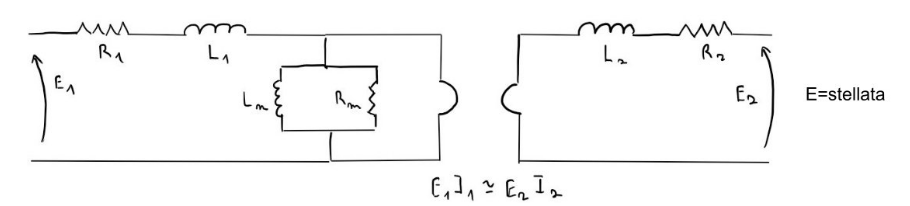
\includegraphics[width=0.8\linewidth]{immagini/cost_prim1}
\end{figure}

Nello studio analitico delle costanti primarie in condizioni di regime permanente sinusoidale si adottano le seguenti ipotesi semplificative di base:
\begin{itemize}
    \item Conduttori cilindrici, rettilinei, indefiniti, paralleli tra loro e paralleli alla superficie del terreno.
    \item Terreno piano, infinitamente esteso, omogeneo, caratterizzato da resistività costante e con permeabilità magnetica relativa $\mu_r = 1$ e costante dielettrica relativa $\varepsilon_r = 1$.
\end{itemize}

\section{Costanti primarie delle linee aeree}
\subsection{Induttanza}
\subsubsection{Induttanza apparente di una linea monofase}
Le correnti che percorrono i conduttori di una linea elettrica sostengono un campo di induzione magnetica nello spazio circostante e all'interno dei conduttori stessi. Il flusso magnetico variabile nel tempo induce forze elettromotrici che si oppongono alla causa generatrice, manifestandosi come cadute di tensione longitudinali lungo i conduttori.

Per disaccoppiare formalmente i conduttori di una linea, si introduce il concetto di \textbf{induttanza apparente} (o coefficiente di autoinduzione apparente): un parametro fittizio per unità di lunghezza che attribuisce a ciascun conduttore un'induttanza propria tale che il comportamento elettrico della singola fase dipenda unicamente dalla corrente che la attraversa, inglobando gli effetti di auto e mutua induzione.
\begin{figure}[H]
	\centering
	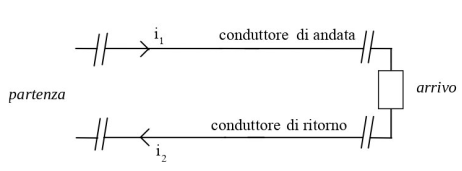
\includegraphics[width=0.5\linewidth]{immagini/cost_prim2}
\end{figure}

Il calcolo dell'induttanza apparente di una linea monofase si riconduce a quello del coefficiente di autoinduzione di una spira indefinita di lunghezza unitaria formata dal conduttore di andata e dal conduttore di ritorno (con $i_1 = i_2 = i$). Il procedimento analitico si articola nelle seguenti fasi:
\begin{enumerate}
    \item \textbf{Legame tra flusso e corrente} $\rightarrow$ La forza elettromotrice indotta nella spira per variazione di flusso magnetico è data da:
    \[e_s = -\frac{d\phi}{dt} = -L \frac{di}{dt}\]
    In condizioni di linearità magnetica dell'aria e del materiale conduttore, il flusso totale $\phi$ concatenato con la spira unitaria (trascurando i tratti terminali di richiusura) è pari alla somma del flusso $\phi_1$ generato dalla corrente nel conduttore 1 e del flusso $\phi_2$ generato dalla corrente nel conduttore 2:
    \[\phi = \phi_1 + \phi_2\]
    Per simmetria geometrica e parità di corrente risulta $\phi_1 = \phi_2$, da cui:
    \[L = \frac{\phi}{i} = \frac{\phi_1 + \phi_2}{i} = \frac{2\phi_1}{i}\]

    \item \textbf{Scomposizione del flusso generato da un singolo conduttore} $\rightarrow$ Il flusso $\phi_1$ sostenuto dal conduttore 1 si scompone in due aliquote:
    \[\phi_1 = \phi_1' + \phi_1''\]
    dove $\phi_1'$ è il flusso esterno concatenato con la porzione di spira compresa tra la superficie esterna del conduttore 1 e l'asse del conduttore 2, mentre $\phi_1''$ è il flusso interno concatenato con la porzione di spira interna al conduttore 1 (tra l'asse e la superficie esterna).

    \item \textbf{Calcolo del flusso esterno $\phi_1'$} $\rightarrow$ Applicando la legge di Biot-Savart, il modulo del campo magnetico alla generica distanza radiale $x'$ dall'asse del conduttore 1 (con $r \le x' \le D$) è dato da:
    \[H_{x'} = \frac{i}{2\pi x'}\]
    L'induzione magnetica corrispondente vale:
    \[B_{x'} = \mu_0 H_{x'} = \mu_0 \frac{i}{2\pi x'}\]
    \begin{figure}[H]
    	\centering
    	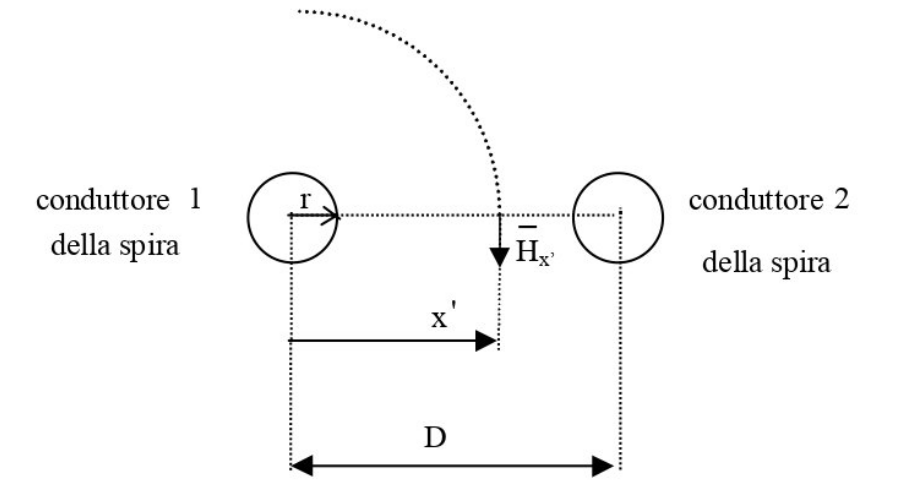
\includegraphics[width=0.6\linewidth]{immagini/cost_prim3}
    \end{figure}
    con $\mu_0 = 4\pi \cdot 10^{-7}\text{ H/m}$. Il vettore induzione magnetica è ortogonale al piano di giacitura della spira elementare di lunghezza unitaria e superficie $dS_{x'} = 1 \cdot dx'$. Il flusso elementare concatenato con tale fascia è:
    \[d\phi_{x'} = B_{x'} \cdot dS_{x'} = 2 \cdot 10^{-7} \frac{i}{x'} \, dx'\]
    Integrando tra il raggio esterno $x' = r$ e l'interasse $x' = D$:
    \[\phi_1' = \int_{r}^{D} 2 \cdot 10^{-7} \frac{i}{x'} \, dx' = 2 \cdot 10^{-7} i \ln\left(\frac{D}{r}\right)\]
    Convertendo ai logaritmi decimali:
    \[\phi_1' = 0{,}46 \cdot 10^{-6} i \log\left(\frac{D}{r}\right)\]

    \item \textbf{Calcolo del flusso interno $\phi_1''$} $\rightarrow$ A distanza $x''$ dal centro del conduttore (con $0 < x'' < r$), il campo magnetico è generato unicamente dalla frazione di corrente $i_{x''}$ racchiusa entro la circonferenza di raggio $x''$:
    \[H_{x''} = \frac{i_{x''}}{2\pi x''}\]
    \begin{figure}[H]
    	\centering
    	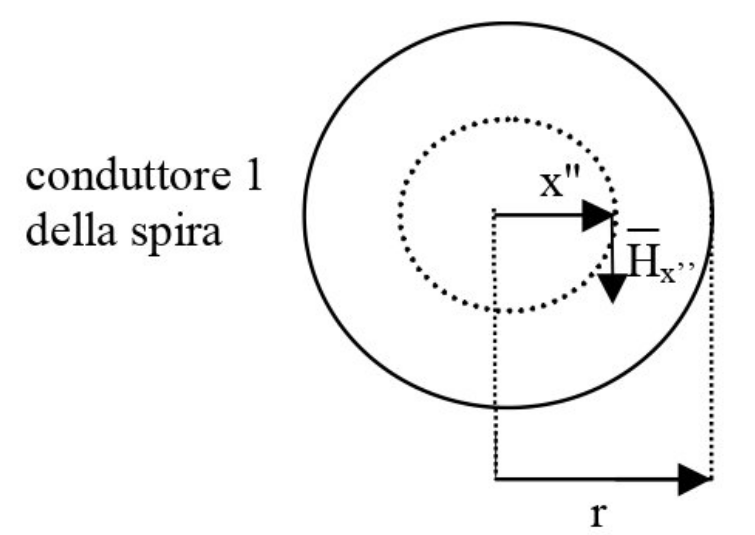
\includegraphics[width=0.4\linewidth]{immagini/cost_prim4}
    \end{figure}
    Ipotizzando distribuzione uniforme della densità di corrente $J$ sulla sezione $S = \pi r^2$ (effetto pelle trascurabile alla frequenza industriale di $50\text{ Hz}$):
    \[J = \frac{i}{\pi r^2} \implies i_{x''} = J \cdot \pi (x'')^2 = i \left(\frac{x''}{r}\right)^2\]
    L'induzione magnetica interna vale:
    \[B_{x''} = \mu_0 \frac{i_{x''}}{2\pi x''} = 2 \cdot 10^{-7} \frac{i (x'')^2}{x'' r^2} = 2 \cdot 10^{-7} \frac{i \, x''}{r^2}\]
    Tale induzione produce un flusso elementare $d\phi_{x''} = B_{x''} (1 \cdot dx'')$ sostenuto unicamente dalla corrente parziale $i_{x''}$. Per calcolare l'induttanza rispetto alla corrente totale $i$, si definisce un flusso equivalente fittizio $d\phi_{x''}^*$ imponendo l'uguaglianza dell'energia magnetica:
    \[i \, d\phi_{x''}^* = i_{x''} \, d\phi_{x''} \implies d\phi_{x''}^* = \frac{i_{x''}}{i} d\phi_{x''} = \left(\frac{x''}{r}\right)^2 \left[2 \cdot 10^{-7} \frac{i \, x''}{r^2} dx''\right] = 2 \cdot 10^{-7} \frac{i}{r^4} (x'')^3 dx''\]
    Integrando tra $x'' = 0$ e $x'' = r$:
    \[\phi_1'' = \int_{0}^{r} 2 \cdot 10^{-7} \frac{i}{r^4} (x'')^3 dx'' = 2 \cdot 10^{-7} \frac{i}{r^4} \left[\frac{(x'')^4}{4}\right]_0^r = 0{,}5 \cdot 10^{-7} i = 0{,}05 \cdot 10^{-6} i\]

    \item \textbf{Flusso totale e induttanza della spira} $\rightarrow$ Sommando i contributi interno ed esterno:
    \[\phi_1 = \phi_1' + \phi_1'' = \left[0{,}05 + 0{,}46 \log\left(\frac{D}{r}\right)\right] 10^{-6} i\]
    \[\phi = 2\phi_1 = 2 \left[0{,}05 + 0{,}46 \log\left(\frac{D}{r}\right)\right] 10^{-6} i\]
    L'induttanza per unità di lunghezza della spira monofase risulta:
    \[L = \frac{\phi}{i} = 2 \left[0{,}05 + 0{,}46 \log\left(\frac{D}{r}\right)\right] \text{ mH/km}\]
    La forza elettromotrice indotta totale nella spira vale:
    \[e_s = -L \frac{di}{dt} = -2 \left[0{,}05 + 0{,}46 \log\left(\frac{D}{r}\right)\right] \frac{di}{dt}\]

    \item \textbf{Disaccoppiamento e induttanza apparente del singolo conduttore} $\rightarrow$ Attribuendo a ciascuno dei due conduttori (andata e ritorno) la metà della forza elettromotrice totale indotta nella spira:
    \[e_c = \frac{e_s}{2} = -\left[0{,}05 + 0{,}46 \log\left(\frac{D}{r}\right)\right] \frac{di}{dt}\]
    si assegna a ciascun conduttore un'induttanza fittizia di autoinduzione, denominata \textbf{induttanza apparente} per unità di lunghezza $L_{am}$:
    \[L_{am} = \frac{L}{2} = 0{,}05 + 0{,}46 \log\left(\frac{D}{r}\right) \quad [\text{mH/km}]\]
\end{enumerate}

Nella relazione di $L_{am}$:
\begin{itemize}
    \item Il termine costante $0{,}05\text{ mH/km}$ rappresenta l'aliquota di autoinduzione interna determinata dal flusso interno al conduttore.
    \item Il termine logaritmico $0{,}46 \log(D/r)\text{ mH/km}$ rappresenta l'aliquota di mutua induzione esterna, dipendente dal rapporto geometrico tra l'interasse $D$ e il raggio $r$.
\end{itemize}

L'induttanza apparente coincide con il rapporto tra un flusso fittizio concatenato col singolo conduttore $\phi_{c1} = \phi/2$ e la corrente che lo attraversa:
\[L_{am} = \frac{\phi_{c1}}{i_1} = \frac{\phi/2}{i} = 0{,}05 + 0{,}46 \log\left(\frac{D}{r}\right)\]
Questo approccio consente di disaccoppiare i conduttori della linea monofase trattandoli singolarmente.

\subsubsection{Induttanza apparente di una finea ad $n$ fasi}
Si consideri un sistema di $n$ conduttori cilindrici rettilinei di raggio $r$, percorsi da correnti equiverse $i_1, i_2, \dots, i_n$ che soddisfano la condizione di equilibrio:
\[\sum_{j=1}^{n} i_j = 0\]
\begin{figure}[H]
	\centering
	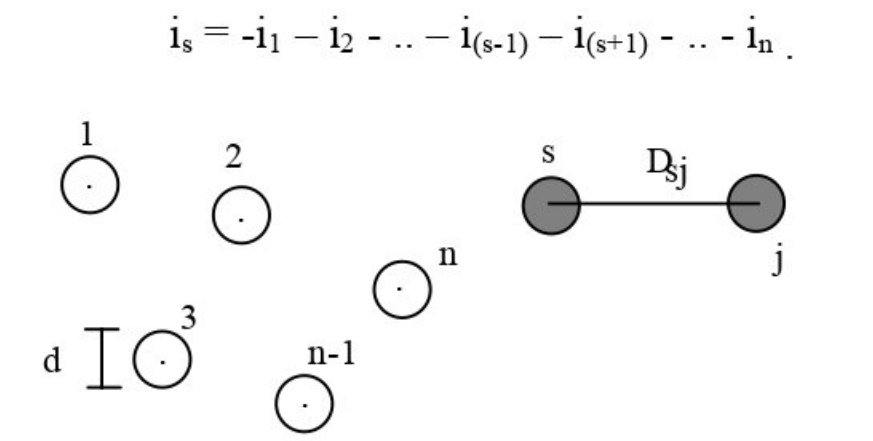
\includegraphics[width=0.5\linewidth]{immagini/cost_prim5}
\end{figure}

Per calcolare l'induttanza apparente del generico conduttore $s$, si esprime la sua corrente come:
\[i_s = -\sum_{j \neq s} i_j\]
Il sistema reale a $n$ conduttori viene sostituito con un sistema fittizio equivalente costituito da $(n-1)$ linee monofasi indipendenti. Ciascuna linea monofase fittizia è formata dal conduttore $s$ (sempre presente) e da uno degli altri conduttori $j$, percorsa dalla corrente $i_j$ nel conduttore $j$ e da $-i_j$ nel conduttore $s$.

Il flusso totale fittizio concatenato con il conduttore $s$ è la somma delle metà dei flussi delle singole linee monofasi:
\[\phi_s = \sum_{j \neq s} \phi_{sj}\]
dove ciascun contributo parziale $\phi_{sj}$, in accordo con il modello monofase, è dato da:
\[\phi_{sj} = \left[0{,}05 + 0{,}46 \log\left(\frac{D_{sj}}{r}\right)\right] (-i_j)\]
Sviluppando la sommatoria ed evidenziando che $\log(D_{sj}/r) = \log(1/r) + \log(D_{sj})$:
\[\phi_s = \sum_{j \neq s} \left[0{,}05 + 0{,}46 \log\left(\frac{1}{r}\right) + 0{,}46 \log(D_{sj})\right] (-i_j)\]
Poiché $\sum_{j \neq s} (-i_j) = i_s$, si ottiene l'espressione generale:
\[\phi_s = \left[0{,}05 + 0{,}46 \log\left(\frac{1}{r}\right)\right] i_s - \sum_{j \neq s} 0{,}46 \log(D_{sj}) \, i_j\]

Nell'espressione del flusso concatenato si individuano:
\begin{itemize}
    \item Un coefficiente fittizio di autoinduzione pari a $[0{,}05 + 0{,}46 \log(1/r)]$ $\rightarrow$ dipende dalla corrente che scorre nel conduttore \textit{s}.
    \item $(n-1)$ coefficienti fittizi di mutua induzione pari a $-0{,}46 \log(D_{sj})$ $\rightarrow$ dipendono dalla corrente che scorre negli altri $n-1$ conduttori.
\end{itemize}

Nel caso generale il flusso $\phi_s$ dipende sia dalla corrente $i_s$ sia dalle correnti circolanti in tutti gli altri conduttori. Non è dunque possibile esprimere il flusso in funzione della sola corrente $i_s$, né ricavare un'induttanza apparente scalare reale che disaccoppi completamente il conduttore dagli altri, a meno di non vincolare le relazioni tra le correnti a specifiche condizioni di simmetria.

\subsubsection{Induttanze di sequenza diretta e inversa in linee trifase}
In un sistema trifase ($n=3$) operante in condizioni di regime sinusoidale simmetrico di sequenza diretta, le correnti di fase costituiscono una terna simmetrica:
\[\bar{I}_1, \quad \bar{I}_2 = \alpha^2 \bar{I}_1, \quad \bar{I}_3 = \alpha \bar{I}_1\]
con l'operatore complesso $\alpha$ e le sue proprietà:
\[\alpha = e^{j \frac{2}{3}\pi} = -\frac{1}{2} + j \frac{\sqrt{3}}{2}, \quad \alpha^2 = e^{j \frac{4}{3}\pi} = -\frac{1}{2} - j \frac{\sqrt{3}}{2}, \quad 1 + \alpha + \alpha^2 = 0\]
\begin{figure}[H]
	\centering
	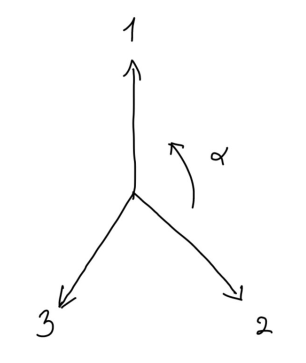
\includegraphics[width=0.25\linewidth]{immagini/cost_prim6}
\end{figure}

Applicando l'espressione generale del flusso al conduttore della fase 1 in forma fasoriale:
\[\bar{\phi}_1 = \left[0{,}05 + 0{,}46 \log\left(\frac{1}{r}\right)\right] \bar{I}_1 - 0{,}46 \log(D_{12}) \bar{I}_2 - 0{,}46 \log(D_{13}) \bar{I}_3\]
Sostituendo $\bar{I}_2 = \alpha^2 \bar{I}_1$ e $\bar{I}_3 = \alpha \bar{I}_1$:
\[\bar{\phi}_1 = \left\{0{,}05 + 0{,}46 \left[\log\left(\frac{1}{r}\right) - \alpha^2 \log(D_{12}) - \alpha \log(D_{13})\right]\right\} \bar{I}_1 = \bar{L}_{a1} \bar{I}_1\]
Il coefficiente di proporzionalità tra flusso e corrente $\bar{L}_{a1}$ è un numero complesso formato da una parte reale e una parte immaginaria:
\[\bar{L}_{a1} = L_{a1R} + j L_{a1I} = 0{,}05 + 0{,}46 \left[\log\left(\frac{1}{r}\right) - \alpha^2 \log(D_{12}) - \alpha \log(D_{13})\right]\]
Sostituendo le espressioni di $\alpha$ e $\alpha^2$:
\[\bar{L}_{a1} = 0{,}05 + 0{,}46 \left[\log\left(\frac{1}{r}\right) + \frac{1}{2}\log(D_{12} D_{13})\right] + j \, 0{,}46 \left[\frac{\sqrt{3}}{2}\log\left(\frac{D_{12}}{D_{13}}\right)\right]\]
Analogamente, per le altre due fasi si ottengono i coefficienti complessi:
\[\bar{L}_{a2} = 0{,}05 + 0{,}46 \left[\log\left(\frac{1}{r}\right) - \alpha^2 \log(D_{23}) - \alpha \log(D_{21})\right]\]
\[\bar{L}_{a3} = 0{,}05 + 0{,}46 \left[\log\left(\frac{1}{r}\right) - \alpha^2 \log(D_{31}) - \alpha \log(D_{32})\right]\]

Le cadute di tensione longitudinali indotte sulle tre fasi risultano:
\[\bar{E}_1 = -j \omega \bar{L}_{a1} \bar{I}_1, \quad \bar{E}_2 = -j \omega \bar{L}_{a2} \bar{I}_2, \quad \bar{E}_3 = -j \omega \bar{L}_{a3} \bar{I}_3\]

\newpage
L'analisi modellistica evidenzia due scenari distinti:
\begin{itemize}
	\item \textbf{Simmetria geometrica} $\rightarrow$ Quando i tre conduttori sono disposti ai vertici di un triangolo equilatero, le distanze mutue sono identiche:
	\[D_{12} = D_{23} = D_{31} = D\]
	\begin{figure}[H]
		\centering
		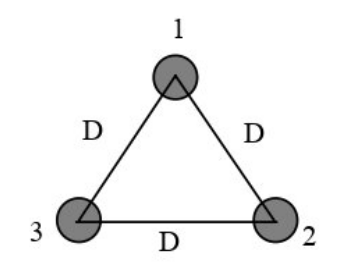
\includegraphics[width=0.3\linewidth]{immagini/cost_prim7}
	\end{figure}
	In condizioni di simmetria geometrica:
	\[\log\left(\frac{D_{12}}{D_{13}}\right) = \log(1) = 0\]
	La parte immaginaria dell'induttanza apparente si annulla identicamente e la parte reale si semplifica in:
	\[\bar{L}_{a1} = \bar{L}_{a2} = \bar{L}_{a3} = L_s = 0{,}05 + 0{,}46 \log\left(\frac{D}{r}\right) \quad [\text{mH/km}]\]
	I coefficienti di proporzionalità sono numeri reali uguali tra loro e coincidenti con l'\textbf{induttanza di servizio} $L_s$. Le cadute di tensione longitudinali sono rigorosamente in quadratura con le rispettive correnti:
	\[\bar{E}_k = -j \omega L_s \bar{I}_k\]
	
	\item \textbf{Dissimmetria geometrica} $\rightarrow$ Nelle configurazioni reali con sostegni troncopiramidali, i conduttori giacciono spesso sullo stesso piano orizzontale o verticale, comportando interdistanze disuguali ($D_{12} = D_{23} \neq D_{13}$).
	\begin{figure}[H]
		\centering
		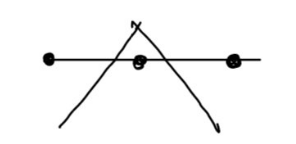
\includegraphics[width=0.3\linewidth]{immagini/cost_prim8}
	\end{figure}
	
	
	La presenza di interdistanze diverse determina:
	\begin{itemize}
		\item La comparsa di una parte immaginaria nell'induttanza apparente, definita \textbf{induttanza obliqua}.
		\item Una caduta di tensione con una componente in quadratura (puramente reattiva) e una componente in fase con la corrente (avente natura formalmente dissipativa o rigenerativa).
		\item L'insorgenza di una terna dissimmetrica di cadute di tensione che, applicata ad una linea alimentata con tensioni di sequenza diretta, genera a fine linea una componente di sequenza inversa, trasformando la terna in una terna spuria.
	\end{itemize}
	
	Per eliminare l'induttanza obliqua e ripristinare la simmetria del sistema, si impiega la tecnica della \textbf{trasposizione dei conduttori}:
	\begin{itemize}
		\item Lo sviluppo complessivo della tratta viene suddiviso in tre sezioni di pari lunghezza.
		\item In ciascuna sezione, ciascun conduttore di fase occupa ciclicamente una delle tre posizioni fisiche nello spazio (rotazione delle fasi).
	\end{itemize}
	\begin{figure}[H]
		\centering
		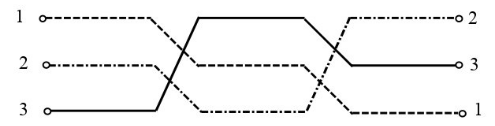
\includegraphics[width=0.6\linewidth]{immagini/cost_prim9}
	\end{figure}
	
	
	L'induttanza obliqua generata in ciascuna sezione si compensa su scala complessiva, annullando la terna inversa di caduta di tensione. Le tre fasi presentano tuttavia induttanze apparenti scalari leggermente diverse tra loro; si definisce pertanto l'\textbf{induttanza di servizio} $L_s$ come la media aritmetica delle induttanze apparenti delle tre tratte:
	\[L_s = \frac{L_{a1} + L_{a2} + L_{a3}}{3} = 0{,}05 + 0{,}46 \log\left(\frac{D_m}{r}\right) \quad [\text{mH/km}]\]
	dove $D_m$ è la distanza media geometrica delle interdistanze:
	\[D_m = \sqrt[3]{D_{12} D_{23} D_{31}}\]
	
	Nelle linee aeree con conduttori nudi, l'induttanza di servizio di sequenza diretta presenta un ordine di grandezza tipico pari a:
	\[L_s \approx 1 \quad [\text{mH/km}]\]
	Alimentando la linea con una terna di tensioni di sequenza inversa, l'induttanza di servizio coincide con quella di sequenza diretta.
\end{itemize}










\subsection{Induttanza di sequenza omopolare}
Quando su una linea trifase si manifestano correnti di sequenza omopolare (innescate da guasti dissimmetrici a terra):
\[\bar{I}_1 = \bar{I}_2 = \bar{I}_3 = \bar{I}_0\]
la corrente risultante pari a $3\bar{I}_0$ non può compensarsi tra le fasi e deve richiudersi attraverso il terreno o le masse metalliche.
\begin{figure}[H]
	\centering
	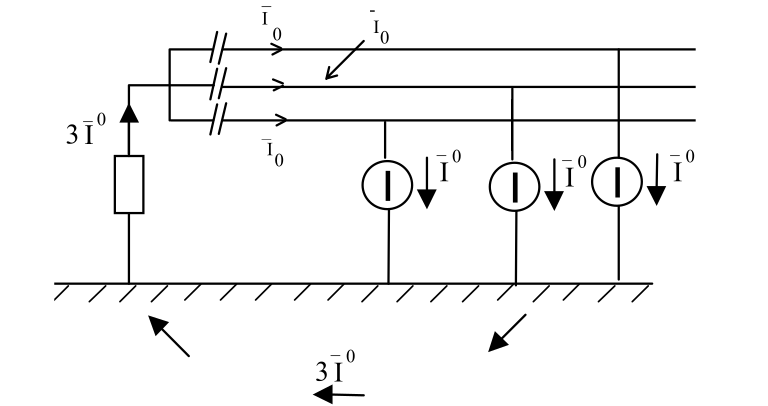
\includegraphics[width=0.6\linewidth]{immagini/cost_prim10}
\end{figure}
Il percorso della corrente nel terreno è governato dalle caratteristiche di conducibilità del suolo e dalla frequenza industriale. La corrente tende ad addensarsi al di sotto della proiezione della linea aerea, distribuendosi in profondità secondo il modello analitico di Carson.

La presenza del terreno viene schematizzata introducendo un \textbf{conduttore immaginario} di ritorno, collocato a una profondità equivalente $D_e$ rispetto ai conduttori di fase, coincidente con il baricentro della distribuzione della corrente:
\[D_e \cong 658 \sqrt{\frac{\rho_t}{f}} \quad [\text{m}]\]
dove $\rho_t$ è la resistività del terreno [$\Omega\cdot\text{m}$] ed $f$ è la frequenza industriale [$\text{Hz}$].
\begin{figure}[H]
	\centering
	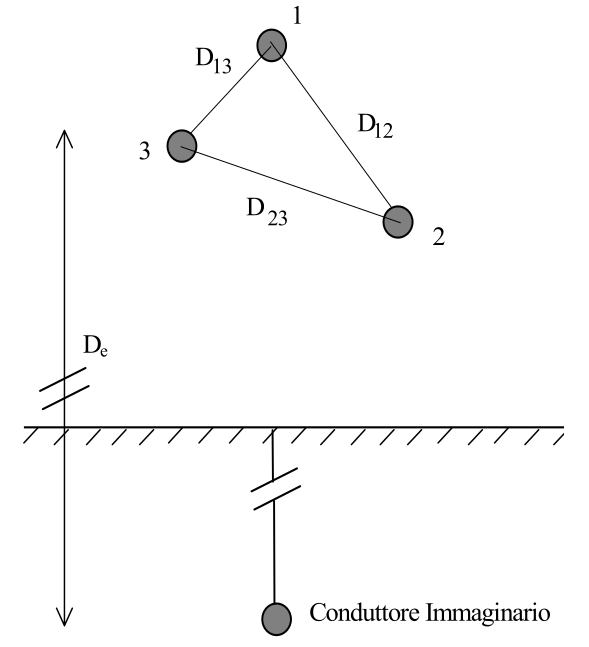
\includegraphics[width=0.4\linewidth]{immagini/cost_prim11}
\end{figure}


Assumendo valori tipici per linee in alta tensione ($\rho_t = 100 \ \Omega\cdot\text{m}$ ed $f = 50\text{ Hz}$):
\[D_e \cong 658 \sqrt{\frac{100}{50}} \approx 930 \quad [\text{m}]\]
L'elevata distanza $D_e$ incrementa sensibilmente il flusso magnetico concatenato con la maglia di ritorno a terra. L'induttanza di sequenza omopolare $L_o$ assume la forma:
\[L_o \cong (3 \div 4) L_s = (3 \div 4) \left[0{,}05 + 0{,}46 \log\left(\frac{D_m}{r}\right)\right] \quad [\text{mH/km}]\]
L'induttanza di sequenza omopolare risulta da 3 a 4 volte superiore rispetto all'induttanza di servizio di sequenza diretta.

In presenza di una o più \textbf{funi di guardia} messe a terra ai sostegni:
\begin{itemize}
    \item La corrente omopolare di ritorno $3\bar{I}_0$ si richiude preferenzialmente attraverso le funi di guardia, attratta dalla loro minore impedenza rispetto al terreno profondo.
    \item La distanza geometrica tra le fasi e le funi di guardia è drasticamente inferiore rispetto alla quota del conduttore fittizio di Carson ($D_e \approx 930\text{ m}$).
    \item L'induttanza di sequenza omopolare si riduce significativamente, assumendo valori prossimi a quelli di sequenza diretta:
    \[L_o \cong (1 \div 1{,}1) L_s\]
\end{itemize}

\subsection{Induttanza in linee trifase con conduttori a fascio}
Nelle linee di trasmissione in alta e altissima tensione (AT e AAT), ciascuna fase viene realizzata mediante conduttori a fascio, costituiti da due, tre o quattro subconduttori elementari mantenuti a distanza prefissata $\Delta$ (tipicamente compresa tra $40\text{ cm}$ e $50\text{ cm}$) tramite distanziatori meccanici.
\begin{figure}[H]
	\centering
	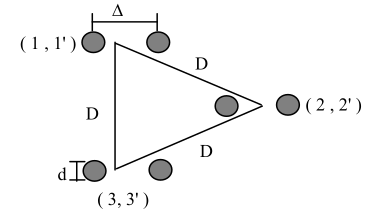
\includegraphics[width=0.3\linewidth]{immagini/cost_prim12}
\end{figure}

I vantaggi dell'adozione dei conduttori a fascio includono:
\begin{itemize}
    \item Riduzione del gradiente di potenziale superficiale sui conduttori, limitando l'innesco dell'effetto corona.
    \item Riduzione dell'induttanza longitudinale di servizio della linea.
    \item Contenimento delle cadute di tensione e aumento del limite di stabilità del sistema elettrico.
\end{itemize}

Per una linea trifase con conduttori a fascio binato (due subconduttori di raggio $r$ a distanza $\Delta$ per ciascuna fase), l'induttanza apparente di fase risulta:
\[L_a = 0{,}025 + 0{,}46 \log\left(\frac{D_m}{r_\Delta}\right) \quad [\text{mH/km}]\]
dove $r_\Delta$ rappresenta il \textbf{raggio equivalente} del fascio binato:
\[r_\Delta = \sqrt{r \Delta}\]
Poiché la distanza tra i subconduttori $\Delta$ è nettamente superiore al raggio fisico $r$, il raggio equivalente risulta notevolmente più grande del raggio del singolo conduttore ($r_\Delta \gg r$). Di conseguenza, l'argomento del logaritmo $D_m/r_\Delta$ decresce sensibilmente, abbattendo l'induttanza di servizio rispetto a una terna a conduttore singolo di pari sezione utile di alluminio. Il termine di autoinduzione interna si dimezza passando da $0{,}05\text{ mH/km}$ a $0{,}025\text{ mH/km}$ per la presenza di due conduttori in parallelo per fase.

\subsection{Capacità}
I conduttori nudi di una linea elettrica si trovano a determinati potenziali elettrici rispetto alla terra e tra di loro, immersi nell'aria che agisce da dielettrico. Si instaurano accoppiamenti elettrostatici tra tutte le coppie di conduttori e tra ciascun conduttore e il suolo, responsabili della circolazione di correnti capacitive trasversali (correnti di spostamento).

Analogamente al caso induttivo, per disaccoppiare elettrostaticamente le fasi si definisce la \textbf{capacità apparente} $C_a$, attribuendo a ciascun conduttore un unico condensatore fittizio verso terra che ingloba tutti gli accoppiamenti mutui e verso il terreno.
\begin{figure}[H]
	\centering
	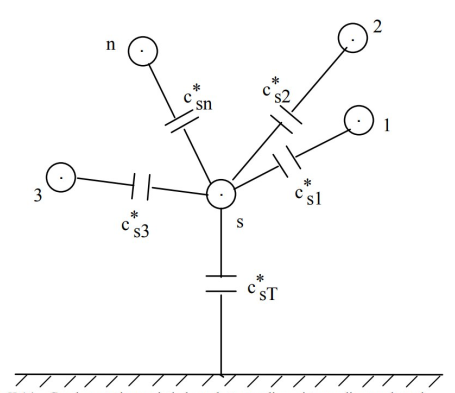
\includegraphics[width=0.4\linewidth]{immagini/cost_prim13}
\end{figure}

In un sistema di $n$ conduttori paralleli ai potenziali $v_1, v_2, \dots, v_n$ rispetto al terreno posto a potenziale nullo ($v_T = 0$), applicando le equazioni di Maxwell la carica per unità di lunghezza distribuita sul generico conduttore $s$ è espressa in funzione delle differenze di potenziale mediante le \textbf{capacità parziali}:
\[Q_s = c_{sT}^* v_s + \sum_{j \neq s} c_{sj}^* (v_s - v_j)\]
dove $c_{sT}^*$ è la capacità parziale del conduttore $s$ verso terra e $c_{sj}^*$ è la capacità parziale mutua tra il conduttore $s$ e il conduttore $j$. Riorganizzando i termini:
\[Q_s = v_s \left(c_{sT}^* + \sum_{j \neq s} c_{sj}^*\right) - \sum_{j \neq s} c_{sj}^* v_j\]

Nel caso generale non è possibile esprimere la carica $Q_s$ in funzione del solo potenziale $v_s$, per cui i conduttori risultano elettrostaticamente accoppiati.

\subsubsection{Capacità di sequenza diretta e inversa in linee trifase}
Considerando una linea trifase ($n=3$) alimentata da una terna simmetrica diretta di tensioni:
\[\bar{V}_1, \quad \bar{V}_2 = \alpha^2 \bar{V}_1, \quad \bar{V}_3 = \alpha \bar{V}_1\]
la carica distribuita sulla fase 1 vale:
\[\bar{Q}_1 = \left[(c_{1T}^* + c_{12}^* + c_{13}^*) - \alpha^2 c_{12}^* - \alpha c_{13}^*\right] \bar{V}_1 = \bar{C}_{a1} \bar{V}_1\]
e analogamente per le fasi 2 e 3:
\[\bar{Q}_2 = \left[(c_{2T}^* + c_{21}^* + c_{23}^*) - \alpha^2 c_{23}^* - \alpha c_{21}^*\right] \bar{V}_2 = \bar{C}_{a2} \bar{V}_2\]
\[\bar{Q}_3 = \left[(c_{3T}^* + c_{31}^* + c_{32}^*) - \alpha^2 c_{31}^* - \alpha c_{32}^*\right] \bar{V}_3 = \bar{C}_{a3} \bar{V}_3\]

In presenza di simmetria geometrica e assumendo che le quote dei conduttori da terra siano molto maggiori delle interdistanze mutue ($H_i \gg D_{ij}$):
\[c_{1T}^* \cong c_{2T}^* \cong c_{3T}^* = c_T, \quad c_{12}^* = c_{23}^* = c_{31}^* = c_m\]
Poiché $1 + \alpha + \alpha^2 = 0$, la capacità apparente scalare risulta identica per le tre fasi:
\[C_{a1} = C_{a2} = C_{a3} = C_a = c_T + 3 c_m\]
Esprimendo la capacità in [$\text{nF/km}$] ed inserendo la permittività dielettrica dell'aria $\varepsilon_0 \approx \frac{10^{-9}}{36\pi}\text{ F/m}$:
\[C_a = \frac{24{,}13}{\log\left(\frac{2D}{d}\right)} \quad [\text{nF/km}]\]
dove $D$ è l'interasse tra i conduttori e $d = 2r$ è il diametro del conduttore. La medesima relazione descrive il funzionamento della linea in condizioni di sequenza inversa.

In assenza di simmetria geometrica, le capacità apparenti $C_{a1}, C_{a2}, C_{a3}$ differiscono tra loro. Ricorrendo alla trasposizione dei conduttori, si introduce la \textbf{capacità di servizio} $C_s$ intesa come media aritmetica delle capacità apparenti:
\[C_s = \frac{C_{a1} + C_{a2} + C_{a3}}{3} = \frac{24{,}13}{\log\left(\frac{2D_m}{d}\right)} \quad [\text{nF/km}]\]
con $D_m = \sqrt[3]{D_{12} D_{23} D_{31}}$. L'ordine di grandezza tipico della capacità di servizio per linee aeree è:
\[C_s \approx 8 \div 10 \quad [\text{nF/km}]\]

\subsubsection{Capacità di sequenza omopolare}
Applicando alla linea trifase una terna di tensioni di sequenza omopolare:
\[\bar{V}_1 = \bar{V}_2 = \bar{V}_3 = \bar{V}_0\]
le differenze di potenziale tra i conduttori di fase si annullano ($v_s - v_j = 0$). Non circolano correnti nelle capacità mutue $c_{sj}^*$ e la carica si disperde esclusivamente attraverso le capacità parziali verso terra $c_{sT}^*$.

Le capacità apparenti omopolari risultano uguali per tutte le fasi:
\[C_o = \frac{24{,}13}{\log\left[\frac{4 H_m}{d} \left(\frac{2 H_m}{D_m}\right)^2\right]} \quad [\text{nF/km}]\]
dove $H_m$ è l'altezza media dei conduttori dal terreno. Numericamente, la capacità di sequenza omopolare risulta pari a circa la metà della capacità di servizio:
\[C_o \approx 0{,}5 \, C_s\]

\subsubsection{Capacità di linee trifase con conduttori a fascio}
Per una linea trifase trasposta con due conduttori a fascio binato per fase, la capacità di servizio assume la forma:
\[C_s = \frac{24{,}13}{\log\left(\frac{2 D_m}{2 \sqrt{r \Delta}}\right)} \quad [\text{nF/km}]\]
La linea con conduttori a fascio binato equivale elettrostaticamente ad una linea a conduttori singoli avente raggio equivalente $r_\Delta = \sqrt{r \Delta}$ (diametro equivalente $d_\Delta = 2\sqrt{r\Delta}$). L'incremento del raggio equivalente produce un aumento della capacità di servizio della linea.

\subsection{Resistenza}
La resistenza elettrica per unità di lunghezza di una linea dipende dalla resistività intrinseca del materiale conduttore, dalla temperatura di esercizio e dalla frequenza della corrente.

La variazione della resistività in funzione della temperatura $T$ rispetto al valore convenzionale a $20^\circ\text{C}$ segue la legge termica:
\[\rho(T) = \rho_{20} [1 + \alpha (T - 20)]\]
I parametri fisici di riferimento dei principali materiali impiegati nelle linee aeree a $20^\circ\text{C}$ sono riassunti nella tabella seguente:

\begin{center}
\begin{tabular}{|l|c|c|}
\hline
\textbf{Materiale} & \textbf{Resistività a $20^\circ\text{C}$ [$\Omega\cdot\text{mm}^2/\text{km}$]} & \textbf{Coefficiente termico $\alpha$ [$^\circ\text{C}^{-1}$]} \\
\hline
Rame & $17{,}8$ & $0{,}0038$ \\
Alluminio & $28{,}3$ & $0{,}0040$ \\
Lega di Aldrey & $32{,}5$ & $0{,}0036$ \\
\hline
\end{tabular}
\end{center}

In regime alternato, la resistenza effettiva è superiore al valore in corrente continua per via della distribuzione disuniforme della corrente nella sezione conduttrice causata da due fenomeni:
\begin{itemize}
    \item \textbf{Effetto pelle} $\rightarrow$ il campo magnetico alternato generato dalla corrente stessa all'interno del conduttore spinge le cariche a concentrarsi in prossimità della superficie esterna, riducendo l'area utile di passaggio.
    \item \textbf{Effetto prossimità} $\rightarrow$ il campo magnetico generato dalle correnti circolanti nei conduttori adiacenti induce una distorsione asimmetrica delle linee di corrente; nelle linee aeree di trasmissione in alta tensione, data la notevole interdistanza geometrica tra i conduttori, l'effetto prossimità risulta trascurabile.
\end{itemize}

Nei \textbf{conduttori bimetallici Alluminio-Acciaio}:
\begin{itemize}
    \item L'alluminio è disposto nella corona circolare esterna, dove si addensa naturalmente la corrente per effetto pelle; l'incremento di resistenza per effetto pelle è perciò più contenuto rispetto a un conduttore monometallico omogeneo.
    \item Nel nucleo centrale di acciaio si generano perdite addizionali nel ferro per isteresi e correnti parassite, funzione della densità di corrente $J$:
    \begin{itemize}
        \item Per $J \le 1\text{ A/mm}^2$ (funzionamento nominale), l'aumento di resistenza non supera l'$1 \div 2\%$.
        \item In condizioni di sovraccarico ($J > 2\text{ A/mm}^2$), le perdite parassite nel nucleo magnetico crescono sensibilmente, aumentando la resistenza effettiva soprattutto in corde di grande diametro.
    \end{itemize}
\end{itemize}

Quando la linea è percorsa da una terna di correnti di sequenza omopolare, il flusso di ritorno $3\bar{I}_0$ interessa il terreno. La presenza del terreno viene modellata mediante il conduttore fittizio di Carson, la cui resistenza per unità di lunghezza è indipendente dalla resistività del terreno e dipende unicamente dalla frequenza industriale:
\[R_T = 3 \cdot 10^{-4} \pi^2 f \quad [\Omega/\text{km}]\]
Alla frequenza di esercizio $f = 50\text{ Hz}$:
\[R_T = 3 \cdot 10^{-4} \pi^2 (50) \approx 0{,}15 \quad [\Omega/\text{km}]\]
La resistenza omopolare totale di ciascuna fase della linea risulta pari a:
\[R_o = R + R_T = R + 0{,}15 \quad [\Omega/\text{km}]\]

\subsection{Conduttanza}
Nelle linee aeree con conduttori nudi, la conduttanza trasversale $g$ modella i fenomeni dissipativi verso l'ambiente esterno legati alla tensione di esercizio, determinati da due contributi:
\begin{itemize}
    \item Le perdite per dispersione superficiale attraverso le catene di isolatori ($P_{is}$).
    \item Le perdite per ionizzazione dell'aria circostante i conduttori dovute all'\textbf{effetto corona} ($P_c$).
\end{itemize}

Indicando con $P_{is}$ e $P_c$ le potenze dissipate per unità di lunghezza e per fase, il valore attribuito alla conduttanza $g$ è dato da:
\[g = \frac{P_{is} + P_c}{V_{nf}^2} \quad [\text{S/km}]\]
essendo $V_{nf}$ il valore efficace della tensione nominale di fase verso terra.

Le perdite negli isolatori $P_{is}$ dipendono dalle condizioni atmosferiche; i loro valori vengono determinati sperimentalmente e forniti dai costruttori.

\subsubsection{Perdite per effetto corona}
Il campo elettrico prodotto dalle cariche sui conduttori è massimo sulla superficie metallica esterna, con intensità inversamente proporzionale al diametro del conduttore. 

Quando il gradiente di potenziale superficiale supera la \textbf{rigidità dielettrica dell'aria} (convenzionalmente assunta pari a $30\text{ kV/cm}$ in aria secca a temperatura e pressione standard), il campo elettrico strappa elettroni alle molecole gassose circostanti, innescando una intensa ionizzazione locale dell'aria denominata \textbf{effetto corona}.

\newpage
L'innesco dell'effetto corona comporta le seguenti conseguenze:
\begin{itemize}
    \item Dissipazione continua di potenza attiva ($P_c$), con peggioramento del rendimento di trasmissione.
    \item Disturbi alle radiofrequenze e alla radioricezione estesi su un ampio spettro elettromagnetico.
    \item Inquinamento acustico continuo (fruscio e schiocchi), particolarmente fastidioso in prossimità di insediamenti abitativi.
    \item Scariche luminose localizzate (bagliori violacei) visibili in condizioni di oscurità.
\end{itemize}

Il campo elettrico critico superficiale $K_c$ necessario per l'innesco del fenomeno dipende dalle condizioni barometriche e ambientali. La potenza dissipata per effetto corona $P_c$ viene valutata mediante la formula empirica di Peek:
\[P_c = \frac{2{,}41}{\delta} (f + 25) \sqrt{\frac{r}{D_m}} (V - V_c)^2 \cdot 10^{-5} \quad [\text{W/km}]\]
dove:
\begin{itemize}
    \item \textbf{$\delta$} $\rightarrow$ fattore di densità relativa dell'aria, definito in funzione della pressione $p$ [$\text{mmHg}$] e della temperatura $t$ [$^\circ\text{C}$]:
    \[\delta = \frac{0{,}392 \, p}{273 + t}\]
    \item \textbf{$V$} $\rightarrow$ valore efficace della tensione del conduttore verso terra [$\text{kV}$].
    \item \textbf{$V_c$} $\rightarrow$ tensione critica verso terra al di sopra della quale si innesca l'effetto corona [$\text{kV}$].
    \item \textbf{$r$} $\rightarrow$ raggio del conduttore [$\text{cm}$].
    \item \textbf{$D_m$} $\rightarrow$ distanza media geometrica dal terreno o tra le fasi [$\text{m}$].
    \item \textbf{$f$} $\rightarrow$ frequenza industriale della tensione di rete ($50\text{ Hz}$).
\end{itemize}

La potenza dissipata cresce quadraticamente rispetto al superamento della tensione critica $(V - V_c)^2$ ed è inversamente proporzionale alla densità dell'aria $\delta$ (aumentando in alta montagna o in climi caldi).

\section{Costanti primarie delle linee in cavo}
Il calcolo delle costanti primarie nelle linee in cavo si basa sui medesimi principi fisici impiegati per le linee con conduttori nudi, ma presenta peculiarità strutturali che modificano radicalmente l'ordine di grandezza e il comportamento dei parametri:
\begin{itemize}
    \item Le interdistanze mutue tra i conduttori di fase e le distanze verso terra sono estremamente ridotte (frazioni di centimetro o pochi centimetri).
    \item Il mezzo dielettrico è costituito da materiali isolanti solidi o fluidi (gomma etilene-propilenica EPR, polietilene reticolato XLPE, carta impregnata) aventi costante dielettrica relativa $\varepsilon_r$ notevolmente superiore a quella dell'aria ($\varepsilon_r \approx 2{,}3 \div 4$).
    \item Il dielettrico solido è sede di perdite dielettriche per polarizzazione ed isteresi, con dissipazioni attive comparabili alle perdite per effetto Joule nei conduttori.
    \item I conduttori sono circondati da schermi, guaine o armature metalliche che costituiscono percorsi conduttivi sede di correnti parassite indotte.
    \item Le correnti omopolari si richiudono preferenzialmente lungo le guaine e gli schermi metallici, anziché nel terreno.
\end{itemize}

\subsection{Induttanza}
Nello studio dell'induttanza dei cavi si distinguono le seguenti condizioni:
\begin{itemize}
    \item \textbf{Cavi tripolari} $\rightarrow$ La simmetria geometrica costruttiva garantisce la coincidenza tra induttanze apparenti e induttanza di servizio. La relazione analitica coincide formalmente con quella delle linee aeree, ma le distanze minime tra i conduttori riducono marcatamente il logaritmo dell'interasse. L'induttanza di servizio risulta da 3 a 4 volte inferiore rispetto a una linea aerea:
    \[L_s \approx 0{,}2 \div 0{,}4 \quad [\text{mH/km}]\]
    (a fronte di $L_s \approx 1\text{ mH/km}$ per linee aeree). L'induttanza omopolare nei cavi tripolari è formalmente identica a quella di una linea aerea con funi di guardia, poiché le correnti omopolari trovano chiusura nelle guaine e armature metalliche contigue.
    \item \textbf{Cavi unipolari schermati} $\rightarrow$ La presenza di correnti indotte nelle guaine metalliche di ciascun cavo determina mutui accoppiamenti complessi; il calcolo analitico richiede formulazioni complesse fornite dai costruttori nei cataloghi tecnici.
\end{itemize}

\subsection{Capacità}
Nelle linee in cavo si distinguono due configurazioni dielettriche fondamentali:

\begin{enumerate}
    \item \textbf{Tre cavi unipolari schermati (o anime a schermo individuale)} $\rightarrow$ Il campo elettrico generato da ciascuna fase è confinato tra il conduttore centrale e lo schermo metallico collegato a terra (campo radiale). Non sussistono accoppiamenti capacitivi mutui tra le fasi ($c_{ij}^* = 0$). La capacità di servizio coincide con la capacità di sequenza omopolare ed è data dalla formula del condensatore cilindrico coassiale:
    \[C_s = C_o = \frac{24{,}13 \, \varepsilon_r}{\log\left(\frac{R}{r}\right)} \quad [\text{nF/km}]\]
    essendo $\varepsilon_r$ la costante dielettrica relativa dell'isolante, $r$ il raggio del conduttore interno ed $R$ il raggio interno dello schermo metallico.

    \item \textbf{Cavo tripolare con unica guaina metallica (a cintura o a campo non radiale)} $\rightarrow$ Il campo elettrico si estende sia tra le singole anime sia tra le anime e la guaina esterna, attivando sia le capacità mutue sia le capacità verso terra. Applicando le relazioni di campo:
    \[C_s = \frac{48{,}26 \, \varepsilon_r}{\log\left[\frac{R^2 - \delta_1^2}{R r}\right] - \log\left[\frac{1}{3}\left(\frac{\delta_1^2}{R^2}\right)^2 + \frac{\delta_1^2}{R^2} + 1\right]} \quad [\text{nF/km}]\]
    \[C_o = \frac{24{,}13 \, \varepsilon_r}{\log\left[\frac{R^2 - \delta_1^2}{R r}\right] + 2 \log\left[\frac{\delta_1^2}{R^2} - 1\right] + \log\left[\frac{1}{4}\left(\frac{\delta_1^2}{R^2}\right)^2 + \frac{\delta_1^2}{R^2} + 1\right]} \quad [\text{nF/km}]\]
    dove $\delta_1$ è il raggio della circonferenza su cui sono disposti i centri dei tre conduttori.
\end{enumerate}
\begin{figure}[H]
	\centering
	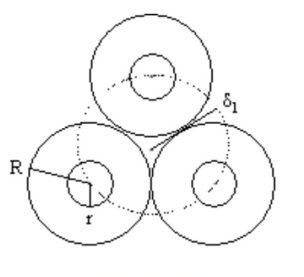
\includegraphics[width=0.3\linewidth]{immagini/cost_prim14}
\end{figure}

Le capacità di servizio nelle linee in cavo risultano nettamente superiori a quelle delle linee aeree:
\begin{itemize}
    \item Piccolissima distanza tra i conduttori e verso terra/schermo.
    \item Maggiore permittività dielettrica relativa dell'isolante solido ($\varepsilon_r > 1$).
\end{itemize}
L'ordine di grandezza tipico della capacità di servizio nei cavi è:
\[C_s \approx 0{,}15 \div 0{,}30 \quad [\mu\text{F/km}]\]
pari a circa $20 \div 30$ volte la capacità di una linea aerea corrispondente.

\subsection{Resistenza}
I principi di calcolo della resistenza ricalcano quelli delle linee aeree, ma presentano un sensibile incremento della resistenza in corrente alternata dovuto a:
\begin{itemize}
    \item Marcato \textbf{effetto prossimità}, innescato dalla stretta vicinanza geometrica tra i conduttori di fase racchiusi nello stesso cavo o posati in fascio.
    \item Perdite addizionali di potenza attiva causate dalla circolazione di correnti parassite indotte nelle guaine, negli schermi e nelle armature metalliche ferromagnetiche.
\end{itemize}

\subsection{Conduttanza}
Nelle linee in cavo l'effetto corona è totalmente assente, essendo i conduttori completamente annegati entro schermi semiconduttivi e dielettrici continui. 

Le dissipazioni di potenza attiva trasversali sono dovute a:
\begin{itemize}
    \item Correnti di conduzione attraverso la resistività volumica finita dell'isolante.
    \item Perdite dielettriche per polarizzazione e isteresi dielettrica nel materiale solido sottoposto a campo alternato, quantificate dal fattore di perdita dielettrica $\tan\delta$:
    \[P_d = \omega C V^2 \tan\delta\]
\end{itemize}
Nei cavi per alta ed altissima tensione, le perdite dielettriche nell'isolante raggiungono entità confrontabili con le perdite per effetto Joule generate nei conduttori dal transito della corrente nominale.

\section{Analisi parametrica e dati di targa dei cavi MT}
Nelle applicazioni ingegneristiche e progettuali relative a cavi di media tensione (MT) isolati, i parametri elettrici vengono reperiti direttamente dalle tabelle fornite dai costruttori:

\begin{itemize}
    \item \textbf{Resistenza apparente a $50\text{ Hz}$ e $90^\circ\text{C}$} $\rightarrow$ All'aumentare della sezione nominale del conduttore ($S$), la resistenza decresce in modo inversamente proporzionale. A parità di sezione nominale ridotta, la resistenza presenta variazioni trascurabili al variare della tensione nominale di isolamento del cavo.
    \item \textbf{Reattanza di fase a $50\text{ Hz}$} $\rightarrow$ I costruttori forniscono direttamente la reattanza di fase $X = \omega L$ [$\Omega/\text{km}$] anziché l'induttanza, poiché è la reattanza ad essere impiegata nei modelli circuitali alla frequenza industriale di $50\text{ Hz}$. La reattanza:
    \begin{itemize}
        \item Diminuisce al crescere della sezione del conduttore, poiché l'aumento del raggio $r$ riduce il valore del termine logaritmico $\log(D/r)$.
        \item Aumenta all'aumentare della tensione nominale di isolamento del cavo, poiché a parità di sezione conduttrice è necessario incrementare lo spessore dell'isolante estruso, allontanando lo schermo metallico o le altre fasi e aumentando il rapporto geometrico $D/r$.
    \end{itemize}
    \item \textbf{Capacità a $50\text{ Hz}$} $\rightarrow$ All'aumentare della sezione geometrica del conduttore, la capacità di servizio aumenta per la maggiore superficie elettrostatica attiva. Sussistono differenze tra cavi schermati e cavi armati, legate alla conformazione geometrica delle armature e alla richiusura delle linee di flusso elettrostatico.
\end{itemize}

\begin{figure}[H]
	\centering
	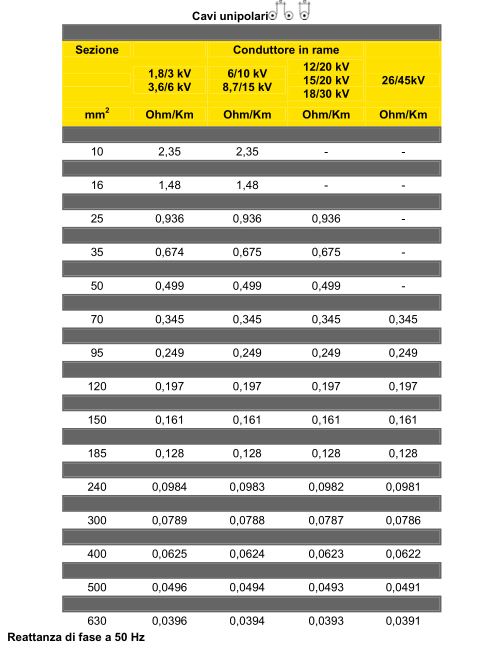
\includegraphics[width=0.6\linewidth]{immagini/cost_prim15}
\end{figure}

\begin{figure}[H]
	\centering
	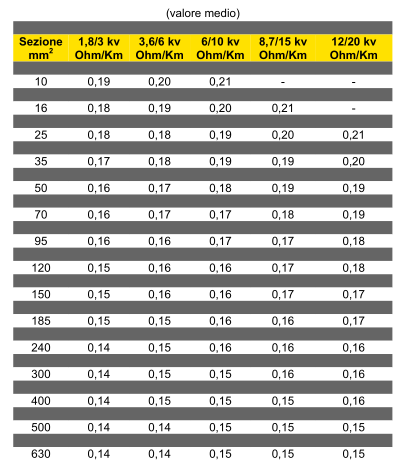
\includegraphics[width=0.55\linewidth]{immagini/cost_prim16}
\end{figure}

\begin{figure}[H]
	\centering
	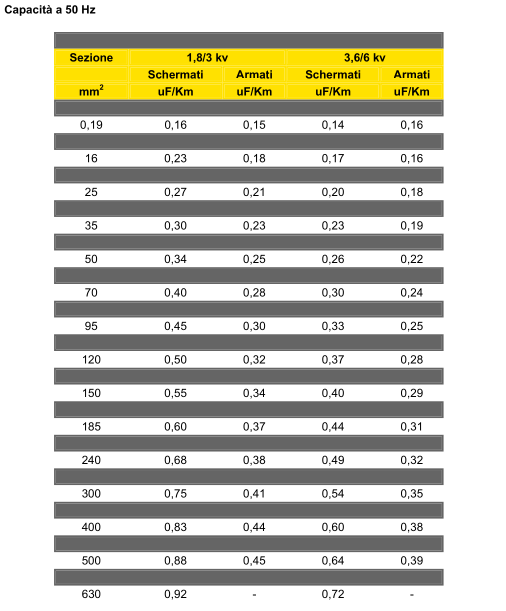
\includegraphics[width=0.6\linewidth]{immagini/cost_prim17}
\end{figure}
